% Lecture Template for ME3001-001-Tristan Hill - Spring 2017 - Fall 2017 - Fall 2020
% Mechanical Engineering Analysis with MATLAB
% Module 2 - Non-Linear Equations
% Topic 4 - The Secant Method

% Document settings

%\documentclass{beamer}                  % for presentation ?
\documentclass[handout]{beamer}  % for handout ?
\usepackage{beamerthemesplit}
\usepackage{amsmath}
\usepackage{listings}
\usepackage{multicol}
\usepackage{framed}
\usepackage{amsmath, nccmath}
\usepackage{geometry}
\usepackage{bm}

\beamertemplateballitem

\definecolor{TTUpurple}{rgb}{0.3098, 0.1607, 0.5176} % TTU Purple (primary)
\definecolor{TTUgold}{rgb}{1.0000, 0.8666, 0.0000} % TTU Gold (primary)

\setbeamercolor{palette primary}{bg=TTUpurple,fg=TTUgold}
\setbeamercolor{palette secondary}{bg=black,fg=TTUgold}
\setbeamercolor{palette tertiary}{bg=black,fg=TTUpurple}
\setbeamercolor{palette quaternary}{bg=TTUgold,fg=black}
\setbeamercolor{structure}{fg=TTUpurple} % itemize, enumerate, etc
\setbeamercolor{section in toc}{fg=TTUpurple} % TOC sections

% custom colors
\definecolor{TTUpurple}{rgb}{0.3098, 0.1607, 0.5176} % TTU Purple (primary)
\definecolor{TTUgold}{rgb}{1.0000, 0.8666, 0.0000} % TTU Gold (primary) 
\definecolor{mygray}{rgb}{.6, .6, .6}
\definecolor{mypurple}{rgb}{0.6,0.1961,0.8}
\definecolor{mybrown}{rgb}{0.5451,0.2706,0.0745}
\definecolor{mygreen}{rgb}{0, .39, 0}
\definecolor{mypink}{rgb}{0.9960, 0, 0.9960}

% color commands
\newcommand{\R}{\color{red}}
\newcommand{\B}{\color{blue}}
\newcommand{\BR}{\color{mybrown}}
\newcommand{\K}{\color{black}}
\newcommand{\G}{\color{mygreen}}
\newcommand{\PR}{\color{mypurple}}
\newcommand{\PN}{\color{mypink}}
\newcommand{\OR}{\color{orange}}
\newcommand{\GD}{\color{TTUgold}}


\newcommand{\Lagr}{\mathcal{L}} % lagrangian

\newcommand{\hspcu}{\underline{\hspace{20mm}}} % large horizontal space w underline
\newcommand{\vspccc}{\vspace{6mm}\\} % large vertical space
\newcommand{\vspcc}{\vspace{4mm}\\}   % medium vertical space
\newcommand{\vspc}{\vspace{2mm}\\}     % small vertical space

\newcommand{\hspcccc}{\hspace{10mm}} % large horizontal space
\newcommand{\hspccc}{\hspace{6mm}} % large horizontal space
\newcommand{\hspcc}{\hspace{4mm}}   % medium horizontal space
\newcommand{\hspc}{\hspace{2mm}}     % small horizontal space

\newsavebox{\mybox} % custom box

\newcommand{\MNUM}{2\hspace{2mm}} % Module number
\newcommand{\TNUM}{4\hspace{2mm}} % Topic number 
\newcommand{\moduletitle}{Nonlinear Equations} % Titles and Stuff
\newcommand{\topictitle}{The Secant Method} 

\newcommand{\sectiontitleI}{What is Secant?} % More Titles and Stuff
\newcommand{\sectiontitleII}{Modified Newton-Raphson }
\newcommand{\sectiontitleIII}{---}
\newcommand{\sectiontitleIV}{A Better Hammer!}

\author{ME3001 - Mechanical Engineering Analysis}
\title{Module \MNUM - \moduletitle}
\date{Mechanical Engineering\vspc Tennessee Technological University}

\begin{document}

\lstset{language=MATLAB,basicstyle=\ttfamily\small,showstringspaces=false}

\frame{\titlepage \center\begin{framed}\Large \textbf{Topic \TNUM - \topictitle}\end{framed} \vspace{5mm}}

% Section 0 - Outline
\frame{
	
	\large \textbf{Topic \TNUM - \topictitle} \vspace{3mm}\\
	
	\begin{itemize}
	
		\item \sectiontitleI    \vspc % Section I
		\item \sectiontitleII 	\vspc % Section II
		\item \sectiontitleIII 	\vspc %Section III
		\item \sectiontitleIV 	\vspc %Section IV
	
	\end{itemize}

}


\section{\sectiontitleI}

\frame{
  \frametitle{\sectiontitleI}
  
	\textbf{What does \PR{secant} \K mean?} \vspace{10mm}\\
	\textbf{The Newton-Raphson method is not \PR{purely numerical}\K, why?} \\
		\begin{itemize}
			\item  The Equation\vspace{3mm}	\\
			\item  The Derivation\vspace{3mm}	\\
		\end{itemize}
	\textbf{How can we avoid this issue?}\\

	
} 

\section{\sectiontitleII}

\frame{
  \frametitle{\sectiontitleI}
  
	\textbf{The {\PR secant} method is a modified version of the Newton-Raphson method.} \vspace{10mm}\\
\textbf{What are the benefits?} \\
		\begin{itemize}
			\item  \vspace{3mm}
			\item  \vspace{3mm}	
		\end{itemize}


} 
\end{document}

%\begin{itemize}
%\Large
%	\item \textbf{What does \PR{secant} \K mean?} \vspace{30mm}\\
%	\item \textbf{The Newton-Raphson method is not \PR{purely numerical}\K, why?} \\\\
%		\begin{itemize}
%			\item  The Equation\vspace{30mm}	\\
%			\item  The Derivation\vspace{30mm}	\\
%		\end{itemize}
%	\item \textbf{\LARGE  How can we avoid this issue?}\\\\
%
%\newpage
%	\item \textbf{ \LARGE Introduce the {\it Secant Method (modified Newton-Raphson)}}
%\begin{itemize}	
%	\item \LARGE{Forward Difference}\\\\
%	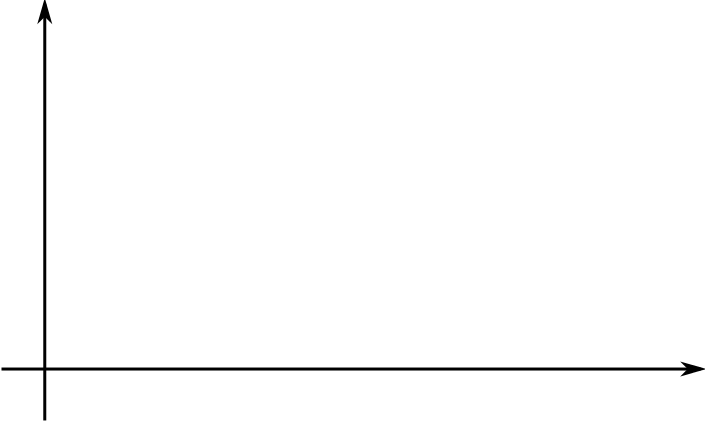
\includegraphics[scale=.35]{lecture4_fig1.png}\\
%	\item \LARGE{Backwards Difference}\\\\
%	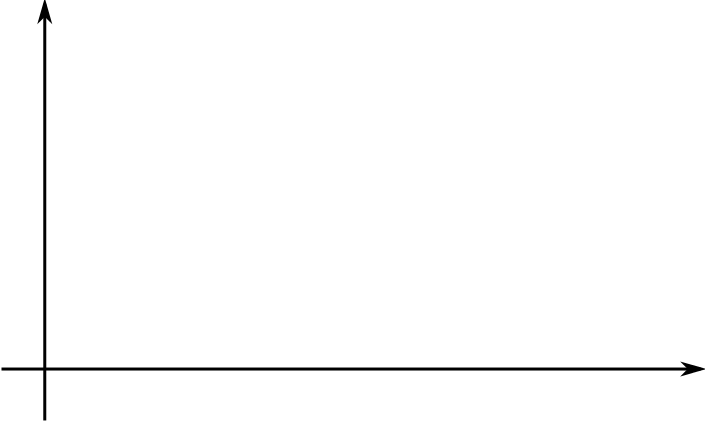
\includegraphics[scale=.35]{lecture4_fig1.png}\\
%	\item \LARGE{Central Difference}\\\\
%	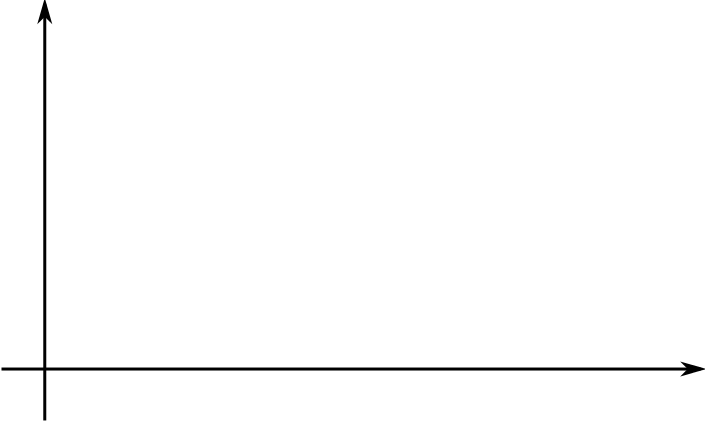
\includegraphics[scale=.35]{lecture4_fig1.png}
%\newpage
%	\item \LARGE{These are know as {\it Finite Difference Approximations} .}\\
%	\item \LARGE{When they are used in the {\it Newton-Raphson} equation this becomes the {\it Secant Method} .}\vspace{25mm}\\
%	
%	\item \LARGE{So what is different about using this method? }\\
%		
%\end{itemize}
%
%		\newpage
%
%\end{itemize}
%\newpage 
%
%% part 2 of the lecture
%\textbf{ \LARGE A Brief Introduction to Optimization } \\
%
%\begin{itemize}
%\Large
%	\item \textbf{\LARGE What is Optimization ?}
%		\begin{itemize}
%			\item Find Local Minima and Maxima \vspace{80mm}	
%			\item Constraints	
%		\end{itemize}
%		\newpage
%		
%	\item \textbf{\LARGE Root finding and Optimization?}
%		\begin{itemize}
%			\item Using the derivative, 4$^{th}$ form of the problem... \vspace{80mm}	
%	
%		\end{itemize}
%	\item \textbf{\LARGE What kind of problems do we solve? Think about the cone we designed a few days ago.}	\\
%			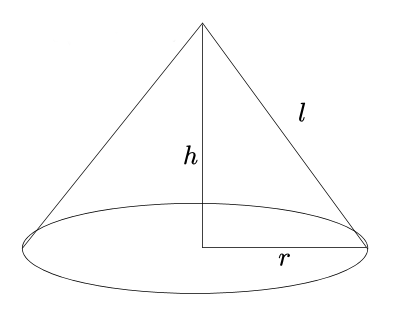
\includegraphics[scale=.5]{lecture4_fig3.png}\hspace{5mm}
%		 \scalebox{1.2}{surface area, $s=\pi r l = \pi r \sqrt{h^2+r^2}$} \\\\
%		  \hspace*{60mm} \scalebox{1.2}{volume, $v=\pi r^2 \frac{h}{3}$} \\\\
%		
%		\newpage
%
%	\item \textbf{\LARGE Optimization Techniques}\\\\
%		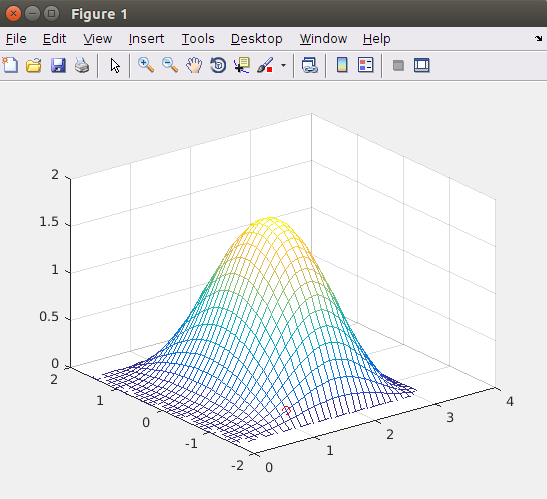
\includegraphics[scale=1]{lecture4_fig2.png}
%		\begin{itemize}
%			\item Brute Force \vspace{30mm}
%			\item Steepest Accent	
%		\end{itemize}
%		\newpage
%
%\end{itemize}
%\textbf{ \LARGE REMINDERS } \\
%
%\begin{itemize}
%
%	\item \textbf{ \LARGE Homework was due Friday but there is a late policy.} \\
%	
%	\item \textbf{ \LARGE The late policy has changed slightly. Please see the syllabus} \\
%	 
%	\item \textbf{ \LARGE MATLAB script from today's lecture will be posted on ilearn. } \\
%		
% \end{itemize}
%
%
%
%
%	
%
%\end{document}
%
%
%
%
%
